\documentclass[aspectratio=169,10pt]{beamer}

% --- Theme & Styling ---
\usetheme{Madrid}
\usecolortheme{beaver}

\setbeamertemplate{navigation symbols}{}
\setbeamertemplate{caption}[numbered]
\setbeamertemplate{footline}[frame number]

% --- Packages ---
\usepackage[utf8]{inputenc}
\usepackage[T1]{fontenc}
\usepackage{amsmath,amssymb,amsfonts}
\usepackage{booktabs}
\usepackage{multirow}
\usepackage{multicol}
\usepackage{graphicx}
\usepackage{tikz}
\usepackage{xcolor}
\usepackage{colortbl}

% --- Custom Colors ---
\definecolor{navyblue}{RGB}{20, 35, 60}
\definecolor{crimsonred}{RGB}{160, 30, 45}
\definecolor{slatepurple}{RGB}{85, 65, 115}
\definecolor{softgray}{RGB}{245, 247, 250}
\definecolor{cardbg}{RGB}{235, 240, 245}

\setbeamercolor{structure}{fg=crimsonred}
\setbeamercolor{frametitle}{fg=white, bg=navyblue}
\setbeamercolor{title}{fg=white, bg=navyblue}

% --- Title Information ---
\title[Crime Analytics Suite]{Crime Intelligence \& Geospatial Analytics Suite}
\subtitle{Big Data Analytics (BDA) Project — NCRB 2024 National \& Metropolitan Study}
\author[BDA Project Team]{Big Data Analytics Project}
\institute[NCRB 2024 Analysis]{
    Department of Computer Science \& Data Analytics \\
    National Crime Records Bureau (NCRB) 2024 Dataset Analysis
}
\date{\today}

\begin{document}

% ==============================================================================
% SLIDE 1: TITLE SLIDE (Page 1)
% ==============================================================================
\begin{frame}[plain]
    \titlepage
\end{frame}

% ==============================================================================
% SLIDE 2: EXECUTIVE SUMMARY & PROBLEM MOTIVATION (Page 2)
% ==============================================================================
\begin{frame}{1. Problem Statement \& Research Motivation}
    \begin{columns}[T]
        \begin{column}{0.48\textwidth}
            \begin{block}{Challenges in NCRB Crime Registries}
                \begin{itemize}
                    \item \textbf{High Spatial Skew:} Small subset of districts accounts for disproportionately high crime volumes.
                    \item \textbf{State Reporting Disparities:} Variation in categorization and chargesheeting standards across states.
                    \item \textbf{Dimensional Complexity:} Hundreds of overlapping categories spanning IPC, SLL, cyber, and vulnerable populations.
                \end{itemize}
            \end{block}
        \end{column}
        \begin{column}{0.48\textwidth}
            \begin{block}{Project Objectives \& Scope}
                \begin{itemize}
                    \item \textbf{Dual-Tier Framework:} Decouple 964 rural/urban districts from 37 million-plus metropolitan cities.
                    \item \textbf{Unsupervised ML:} Apply PCA, K-Means clustering, and DBSCAN anomaly detection.
                    \item \textbf{Policy Intelligence:} Benchmark metropolitan policing efficiency and decompose crime motives.
                    \item \textbf{Deployment:} Glassmorphic interactive dashboard with LLM-powered query assistant.
                \end{itemize}
            \end{block}
        \end{column}
    \end{columns}

    \vspace{0.3cm}
    \begin{alertblock}{Key Analytical Scope}
        Covering \textbf{964 Districts} across \textbf{36 States/UTs} and \textbf{37 Metropolitan Cities} (NCRB 2024 Release).
    \end{alertblock}
\end{frame}

% ==============================================================================
% SLIDE 3: DUAL-TIER DATA ARCHITECTURE (Page 3)
% ==============================================================================
\begin{frame}{2. Dual-Tier Data Architecture \& Curation}
    \begin{table}[h]
        \centering
        \small
        \caption{Curated Data Portfolio (17 Total Audited Datasets)}
        \rowcolors{2}{softgray}{white}
        \begin{tabular}{lllp{6cm}}
            \toprule
            \textbf{Tier} & \textbf{Scope} & \textbf{Files} & \textbf{Key Analytical Dimensions Covered} \\
            \midrule
            \textbf{Tier 1} & District Core & 9 Files & IPC Crimes, SLL, Women Safety, Child Protection, SC/ST Atrocities, Juvenile Delinquency, Cybercrime, Missing Persons. \\
            \midrule
            \textbf{Tier 2} & Metropolitan & 8 Files & 3-Year Trends (2022--2024), Chargesheeting Rates, Murder Motives (35), Cyber Motives (25), Juvenile Demographics \& Socioeconomics. \\
            \bottomrule
        \end{tabular}
    \end{table}

    \begin{columns}[T]
        \begin{column}{0.48\textwidth}
            \begin{block}{Portfolio Audit \& Verification}
                \begin{itemize}
                    \item Programmatic validation via \texttt{curated\_loader.py}.
                    \item Verification of row/column schemas and zero file missingness.
                \end{itemize}
            \end{block}
        \end{column}
        \begin{column}{0.48\textwidth}
            \begin{block}{Master Matrix Scale}
                \begin{itemize}
                    \item \textbf{District Matrix:} $964 \times 696$ feature dimensions.
                    \item \textbf{Metro Matrix:} $37 \times 18$ efficiency metrics.
                \end{itemize}
            \end{block}
        \end{column}
    \end{columns}
\end{frame}

% ==============================================================================
% SLIDE 4: PREPROCESSING & DATA CLEANING PIPELINE (Page 4)
% ==============================================================================
\begin{frame}{3. Data Preprocessing \& Cleaning Pipeline}
    \begin{columns}[T]
        \begin{column}{0.55\textwidth}
            \begin{block}{Complexities Resolved in Raw NCRB Excel Files}
                \begin{enumerate}
                    \item \textbf{Multi-Row Hierarchical Headers:} Rows 1--3 contain nested column descriptions; resolved via custom \texttt{openpyxl} parser.
                    \item \textbf{Embedded State Headers:} Interspersed subtotal rows (e.g., \textit{"State: Uttar Pradesh"}) extracted into dedicated \texttt{state} columns.
                    \item \textbf{Text-Numeric Contamination:} Asterisks, footnote labels (\textit{e.g.,} \texttt{[1]}, \texttt{*}, \texttt{+}), and non-standard missing flags (\texttt{-}, \texttt{NA}, \texttt{N.A.}) sanitized to numerical zero.
                    \item \textbf{District Normalization:} State and district names standardized using fuzzy string mapping.
                \end{enumerate}
            \end{block}
        \end{column}
        \begin{column}{0.42\textwidth}
            \begin{block}{Data Processing Pipeline}
                \centering
                \tikzstyle{startstop} = [rectangle, rounded corners, minimum width=2.5cm, minimum height=0.6cm,text centered, draw=black, fill=cardbg]
                \begin{tikzpicture}[node distance=1.1cm]
                    \node (raw) [startstop] {\textbf{Raw NCRB Excel Files}};
                    \node (parse) [startstop, below of=raw] {Custom \texttt{openpyxl} Parser};
                    \node (clean) [startstop, below of=parse] {Clean Domain Parquets};
                    \node (master) [startstop, below of=clean] {\textbf{Master Feature Matrix}};
                    \draw [->, thick] (raw) -- (parse);
                    \draw [->, thick] (parse) -- (clean);
                    \draw [->, thick] (clean) -- (master);
                \end{tikzpicture}
            \end{block}
        \end{column}
    \end{columns}
\end{frame}

% ==============================================================================
% SLIDE 5: FEATURE ENGINEERING & DOMAIN METRICS (Page 5)
% ==============================================================================
\begin{frame}{4. Feature Engineering: 25 Composite Ratios}
    To eliminate scale distortion across varying district sizes, \textbf{25 domain-specific composite indices} were engineered:

    \vspace{0.15cm}
    \begin{columns}[T]
        \begin{column}{0.48\textwidth}
            \begin{block}{Core Violent \& Vulnerability Ratios}
                \footnotesize
                \begin{itemize}
                    \item \textbf{Violent Crime Ratio:}\\[2pt]
                    $\displaystyle\frac{\text{Murder} + \text{Rape} + \text{Kidnap}}{\text{Total IPC Crimes} + \epsilon}$
                    \vspace{0.1cm}
                    \item \textbf{Women Vulnerability Share:}\\[2pt]
                    $\displaystyle\frac{\text{Crimes against Women}}{\text{Total IPC Crimes} + \epsilon}$
                    \vspace{0.1cm}
                    \item \textbf{Child Crime Ratio:}\\[2pt]
                    $\displaystyle\frac{\text{POCSO} + \text{Child Kidnap}}{\text{Total IPC Crimes} + \epsilon}$
                \end{itemize}
            \end{block}
        \end{column}
        \begin{column}{0.48\textwidth}
            \begin{block}{Specialized Risk \& Intensity Scores}
                \footnotesize
                \begin{itemize}
                    \item \textbf{Cyber Intensity Score:}\\[2pt]
                    $\displaystyle\frac{\text{IT Act Offenses}}{\text{Total SLL Crimes} + \epsilon}$
                    \vspace{0.1cm}
                    \item \textbf{Trafficking Proxy:}\\[2pt]
                    $\displaystyle\frac{\text{Missing Children}}{\text{Child Kidnapping} + \epsilon}$
                    \vspace{0.1cm}
                    \item \textbf{Caste Atrocity Index:}\\[2pt]
                    $\displaystyle\frac{\text{SC Crimes} + \text{ST Crimes}}{\text{Total IPC Crimes} + \epsilon}$
                \end{itemize}
            \end{block}
        \end{column}
    \end{columns}

    \vspace{0.15cm}
    \begin{block}{Standardization Protocol}
        \footnotesize
        All engineered features were scaled using \textbf{RobustScaler} (median and IQR normalization) to reduce sensitivity to extreme localized outliers prior to model training.
    \end{block}
\end{frame}

% ==============================================================================
                    %SLIDE 6: DIMENSIONALITY REDUCTION (PCA) (Page 6)
% ==============================================================================
\begin{frame}{5. Dimensionality Reduction via PCA}
    \begin{columns}[T]
        \begin{column}{0.5\textwidth}
            \begin{block}{Mathematical Formulation}
                Given scaled matrix $X \in \mathbb{R}^{964 \times 25}$, Principal Component Analysis computes eigenvectors $v_k$ of covariance matrix $\Sigma$:
                $$\Sigma v_k = \lambda_k v_k$$
                Top 2 principal components capture \textbf{66.8\%} of total feature variance:
                \begin{itemize}
                    \item \textbf{PC1 (42.3\% Variance):} Captures aggregate volume scale across all crime domains.
                    \item \textbf{PC2 (24.5\% Variance):} Discriminates between Violent/Atrocity orientation vs. Cyber/Vulnerability focus.
                \end{itemize}
            \end{block}
        \end{column}
        \begin{column}{0.46\textwidth}
            \begin{block}{PCA Factor Loadings Summary}
                \small
                \rowcolors{2}{softgray}{white}
                \begin{tabular}{lrr}
                    \toprule
                    \textbf{Engineered Feature} & \textbf{PC1} & \textbf{PC2} \\
                    \midrule
                    Total IPC Crimes & \textbf{+0.38} & -0.12 \\
                    Violent Crime Ratio & \textbf{+0.34} & \textbf{+0.41} \\
                    Women Vulnerability Share & +0.29 & \textbf{+0.36} \\
                    Cyber Intensity Score & +0.18 & \textbf{-0.48} \\
                    Caste Atrocity Index & +0.22 & \textbf{+0.33} \\
                    Property Crime Share & +0.31 & -0.21 \\
                    \bottomrule
                \end{tabular}
            \end{block}
        \end{column}
    \end{columns}
\end{frame}

% ==============================================================================
% SLIDE 7: UNSUPERVISED MACHINE LEARNING — K-MEANS (Page 7)
% ==============================================================================
\begin{frame}{6. Machine Learning: K-Means Spatial Clustering}
    \begin{columns}[T]
        \begin{column}{0.48\textwidth}
            \begin{block}{Optimization Objective}
                $$\arg\min_{\mathbf{S}} \sum_{i=1}^{k} \sum_{\mathbf{x} \in S_i} \left\| \mathbf{x} - \boldsymbol{\mu}_i \right\|^2$$
                Evaluated across $k \in \{2, 3, 4, 5, 6, 7, 8\}$ using:
                \begin{itemize}
                    \item \textbf{Elbow Method:} Inertia inflection point.
                    \item \textbf{Silhouette Score:} Peak cluster separation at $k=5$ ($S = 0.442$).
                    \item \textbf{Davies-Bouldin Index:} Minimized at $k=5$ ($DB = 0.812$).
                \end{itemize}
            \end{block}
        \end{column}
        \begin{column}{0.48\textwidth}
            \begin{block}{Evaluation Metrics Matrix}
                \small
                \rowcolors{2}{softgray}{white}
                \begin{tabular}{cccc}
                    \toprule
                    \textbf{k} & \textbf{Inertia} & \textbf{Silhouette} & \textbf{Davies-Bouldin} \\
                    \midrule
                    3 & 14,210 & 0.381 & 0.982 \\
                    4 & 10,850 & 0.412 & 0.894 \\
                    \rowcolor{cardbg}
                    \textbf{5} & \textbf{8,240} & \textbf{0.442} & \textbf{0.812} \\
                    6 & 7,410 & 0.398 & 0.855 \\
                    7 & 6,820 & 0.375 & 0.891 \\
                    \bottomrule
                \end{tabular}
            \end{block}
        \end{column}
    \end{columns}
\end{frame}

% ==============================================================================
% SLIDE 8: SPATIAL TYPOLOGIES ANALYSIS (Page 8)
% ==============================================================================
\begin{frame}{7. Spatial Typologies of Indian Districts}
    \begin{table}[h]
        \centering
        \footnotesize
        \caption{Summary of 5 National District Crime Typologies ($N = 964$)}
        \rowcolors{2}{softgray}{white}
        \begin{tabular}{clccp{5.2cm}}
            \toprule
            \textbf{Cluster} & \textbf{Typology Label} & \textbf{Districts} & \textbf{\% Share} & \textbf{Dominant Crime Characterization} \\
            \midrule
            \textbf{0} & Women \& Child Vulnerability & 170 & 17.6\% & High rape, POCSO, and domestic harassment ratios. \\
            \textbf{1} & Agrarian \& Caste Vulnerable & 577 & 59.8\% & Elevated SC/ST atrocities, property disputes. \\
            \textbf{2} & High-Intensity Urban Hubs & 35 & 3.6\% & High total volume, violent crime, complex IPC. \\
            \textbf{3} & Low-Intensity Baseline & 96 & 10.0\% & Low overall crime burden across all categories. \\
            \textbf{4} & Moderate Mixed-Crime Hubs & 86 & 8.9\% & Cybercrime intensity combined with theft/SLL. \\
            \bottomrule
        \end{tabular}
    \end{table}

    \begin{alertblock}{Key Spatial Finding}
        Over \textbf{59.8\% of Indian districts} belong to Cluster 1 (Agrarian \& Caste Vulnerable), highlighting structural socio-economic drivers behind regional rural crime patterns.
    \end{alertblock}
\end{frame}

% ==============================================================================
% SLIDE 9: DBSCAN ANOMALY DETECTION (Page 9)
% ==============================================================================
\begin{frame}{8. Density-Based Anomaly Detection (DBSCAN)}
    \begin{columns}[T]
        \begin{column}{0.5\textwidth}
            \begin{block}{Algorithm Hyperparameters}
                DBSCAN applied to top Principal Components:
                $$\epsilon = 0.85, \quad MinPts = 5$$
                Districts classified as noise points ($Label = -1$) lack sufficient density neighborhood support:
                $$|N_\epsilon(p)| < MinPts$$
            \end{block}
            \begin{block}{Outlier Characteristics}
                Outlier districts exhibit extreme multi-dimensional crime profiles (e.g., disproportionate cyber fraud spikes or extreme violent ratios).
            \end{block}
        \end{column}
        \begin{column}{0.46\textwidth}
            \begin{block}{Anomaly Detection Results}
                \begin{itemize}
                    \item \textbf{Total Anomalies Identified:} \textbf{28 Districts} (2.9\% of all districts).
                    \item \textbf{Geographic Concentration:} Primary clusters found in industrial corridors and cross-state border districts.
                    \item \textbf{Policy Impact:} Requires targeted audit rather than standard cluster policing.
                \end{itemize}
            \end{block}
        \end{column}
    \end{columns}
\end{frame}

% ==============================================================================
% SLIDE 10: METROPOLITAN POLICING QUADRANT ANALYSIS (Page 10)
% ==============================================================================
\begin{frame}{9. Metropolitan Policing Efficiency Benchmark}
    \begin{columns}[T]
        \begin{column}{0.52\textwidth}
            \begin{block}{4-Quadrant Benchmark Matrix}
                Evaluates \textbf{37 Million-Plus Cities} across:
                \begin{itemize}
                    \item \textbf{X-Axis:} Median Crime Rate per 100k population.
                    \item \textbf{Y-Axis:} Chargesheeting Rate (\%).
                \end{itemize}
            \end{block}
            \scriptsize
            \rowcolors{2}{softgray}{white}
            \begin{tabular}{lp{3.2cm}}
                \toprule
                \textbf{Quadrant} & \textbf{City Profile \& Count} \\
                \midrule
                \textbf{Q1: Critical Bottleneck} & High Crime Rate, Low Chargesheeting (\textbf{6 Cities}). \\
                \textbf{Q2: High Load \& Efficient} & High Crime Rate, High Chargesheeting (\textbf{9 Cities}). \\
                \textbf{Q3: Effective Containment} & Low Crime Rate, High Chargesheeting (\textbf{10 Cities}). \\
                \textbf{Q4: Latent Risk / Under-report} & Low Crime Rate, Low Chargesheeting (\textbf{12 Cities}). \\
                \bottomrule
            \end{tabular}
        \end{column}
        \begin{column}{0.46\textwidth}
            \begin{block}{Policing Matrix Diagram}
                \centering
                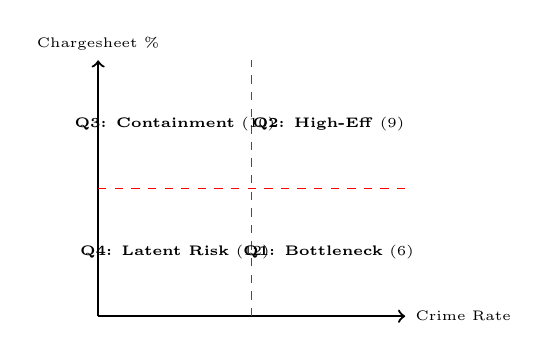
\begin{tikzpicture}[scale=0.65]
                    \draw[->, thick] (0,0) -- (6,0) node[right] {\tiny Crime Rate};
                    \draw[->, thick] (0,0) -- (0,5) node[above] {\tiny Chargesheet \%};
                    \draw[dashed, red] (3,0) -- (3,5);
                    \draw[dashed, red] (0,2.5) -- (6,2.5);
                    \node at (1.5, 3.75) {\tiny \textbf{Q3: Containment} (10)};
                    \node at (4.5, 3.75) {\tiny \textbf{Q2: High-Eff} (9)};
                    \node at (1.5, 1.25) {\tiny \textbf{Q4: Latent Risk} (12)};
                    \node at (4.5, 1.25) {\tiny \textbf{Q1: Bottleneck} (6)};
                \end{tikzpicture}
            \end{block}
        \end{column}
    \end{columns}
\end{frame}

% ==============================================================================
% SLIDE 11: CAUSAL MOTIVE DECOMPOSITION (Page 11)
% ==============================================================================
\begin{frame}{10. Causal Motive Decomposition: Murder \& Cyber}
    \begin{columns}[T]
        \begin{column}{0.48\textwidth}
            \begin{block}{Top Murder Motives (35 Categories)}
                \small
                \rowcolors{2}{softgray}{white}
                \begin{tabular}{lrr}
                    \toprule
                    \textbf{Motive Category} & \textbf{Cases} & \textbf{\% Share} \\
                    \midrule
                    Personal Vendetta / Enmity & 196 & 31.2\% \\
                    Petty Quarrels / Disputes & 177 & 28.2\% \\
                    Property & 94 & 15.0\% \\
                    Illicit Relationships & 68 & 10.8\% \\
                    Gain / Robbery & 35 & 5.6\% \\
                    Organized Gang Rivalry & \textbf{17} & \textbf{2.7\%} \\
                    \bottomrule
                \end{tabular}
            \end{block}
        \end{column}
        \begin{column}{0.48\textwidth}
            \begin{block}{Top Cybercrime Motives (25 Categories)}
                \small
                \rowcolors{2}{softgray}{white}
                \begin{tabular}{lrr}
                    \toprule
                    \textbf{Motive Category} & \textbf{Cases} & \textbf{\% Share} \\
                    \midrule
                    Financial Fraud / Gain & \textbf{3,147} & \textbf{72.4\%} \\
                    Sexual Exploitation & 482 & 11.1\% \\
                    Personal Revenge & 265 & 6.1\% \\
                    Identity Theft & 210 & 4.8\% \\
                    Extortion / Blackmail & 142 & 3.3\% \\
                    \bottomrule
                \end{tabular}
            \end{block}
        \end{column}
    \end{columns}

    \vspace{0.2cm}
    \begin{alertblock}{Empirical Motive Insight}
        Personal disputes drive \textbf{59.4\% of murders} (gang violence is $<3\%$), while financial fraud dominates \textbf{72.4\% of cybercrime}.
    \end{alertblock}
\end{frame}

% ==============================================================================
% SLIDE 12: DASHBOARD & AI ARCHITECTURE (Page 12)
% ==============================================================================
\begin{frame}{11. Production Glassmorphic Dashboard \& AI}
    \begin{columns}[T]
        \begin{column}{0.5\textwidth}
            \begin{block}{Streamlit UI Architecture}
                \begin{itemize}
                    \item \textbf{Glassmorphism Design:} Centralized CSS styling (\texttt{theme.py}) using translucent backdrop blurs and subtle borders.
                    \item \textbf{6 Interactive Views:} Overview, District Explorer, Spatial Clustering, Metropolitan Quadrants, Anomalies, and AI Assistant.
                    \item \textbf{Optimized Caching:} Parquet data loading cached via \texttt{@st.cache\_data}.
                \end{itemize}
            \end{block}
        \end{column}
        \begin{column}{0.46\textwidth}
            \begin{block}{Groq Intelligence Assistant}
                \begin{itemize}
                    \item \textbf{Model:} Groq LLaMA 3.3 70B crime query assistant (\texttt{ai\_assistant.py}).
                    \item \textbf{Strict Guardrails:} Enforces domain-scoped context (NCRB 2024 data only) and rejects non-crime queries.
                    \item \textbf{Fallback Mode:} Graceful fallback when API key is unconfigured.
                \end{itemize}
            \end{block}
        \end{column}
    \end{columns}
\end{frame}

% ==============================================================================
% SLIDE 13: STRATEGIC POLICY MATRIX & CONCLUSION (Page 13)
% ==============================================================================
\begin{frame}{12. Strategic Policy Matrix \& Conclusion}
    \begin{table}[h]
        \centering
        \scriptsize
        \caption{Empirical Finding to Policy Action Matrix}
        \rowcolors{2}{softgray}{white}
        \begin{tabular}{lp{6.5cm}}
            \toprule
            \textbf{Empirical Finding} & \textbf{Targeted Strategic Intervention} \\
            \midrule
            170 Women Vulnerability Districts & Deploy specialized Women \& Child Protection Cells in Cluster 0 districts. \\
            577 Agrarian Caste-Vulnerable Districts & Fast-track PoA Act enforcement and rural dispute resolution mechanisms. \\
            6 Bottleneck Metro Cities (Q1) & Inject forensic capacity and scale up chargesheeting investigation teams. \\
            72.4\% Cybercrime Financial Fraud & Expand specialized digital fraud task forces and banking safety protocols. \\
            28 DBSCAN Anomaly Districts & Initiate targeted state-level data quality and crime reporting audits. \\
            \bottomrule
        \end{tabular}
    \end{table}

    \begin{block}{Project Impact Summary}
        Successfully built an end-to-end Big Data Analytics suite converting \textbf{17 raw NCRB datasets} into actionable intelligence for law enforcement and policy planners.
    \end{block}
\end{frame}

\end{document}
